\documentclass[12pt]{article}
\usepackage[utf8]{inputenc}
\usepackage{geometry}
\usepackage{svg}
\usepackage{float}
\usepackage{caption}
\usepackage{amsmath,amsthm,amsfonts,amssymb,amscd}
\usepackage{fancyhdr}
\usepackage{titlesec}
\usepackage{xparse}
\usepackage{listings}
\usepackage{tikz}
\usepackage{mathtools}
\usepackage[ngerman]{babel}
\usetikzlibrary{shapes.geometric, arrows}
\pagestyle{empty}
\titleformat*{\section}{\large\bfseries}

%
\geometry{
 a4paper,
 total={170mm,240mm},
 left=20mm,
 top=30mm,
 }

\date{}
%Bitte ausfüllen
\newcommand\course{Programmierung, Gruppe 16}
\newcommand\hwnumber{7}
\newcommand\Name{Maximilian Petri, 405602}
\newcommand\Neptun{Danje Petersen, 379748}

%Matheinheiten
\newcommand\m{\:\textrm{m}}
\newcommand\M{\:\Big[\textrm{m}\Big]}
\newcommand\mm{\:\textrm{mm}}
\newcommand\MM{\:\Big[\textrm{mm}\Big]}
\newcommand\un{\underline}
\newcommand\s{\:\textrm{s}}
\newcommand\bS{\:\Big[\textrm{S}\Big]}
\newcommand\ms{\:\frac{\textrm{m}}{\textrm{s}}}
\newcommand\MS{\:\Big[\frac{\textrm{m}}{\textrm{s}}\Big]}
\newcommand\mss{\:\frac{\textrm{m}}{\textrm{s}^2}}
\newcommand\MSS{\:\Big[\frac{\textrm{m}}{\textrm{s}^2}\Big]}
\DeclarePairedDelimiter\ceil{\lceil}{\rceil}
\DeclarePairedDelimiter\floor{\lfloor}{\rfloor}

%Einstellungen für lstlisting
\lstset{
basicstyle=\fontsize{9}{10}\selectfont\ttfamily, 
keywordstyle=\color{purple}\bfseries,           % keywords purple
commentstyle=\color{gray},                     % white comments
stringstyle=\color{blue},                       % strings blue
showstringspaces=false,
language= java}                          % typewriter type for strings                       


%Bitte nicht einstellen

\renewcommand{\thesection}{Aufgabe }
\renewcommand{\thesubsection}{\alph{subsection})}
\renewcommand{\thesubsubsection}{\hspace{0.8cm}\roman{subsubsection})}
\renewcommand{\figurename}{Abbildung}
\renewcommand{\tablename}{Tabelle}
\pagestyle{fancyplain}
\headheight 35pt
\lhead{\Name\\\Neptun}
\chead{\textbf{\Large Hausaufgabe \hwnumber}}
\rhead{\course \\ \today}
\lfoot{}
\cfoot{}
\rfoot{\small\thepage}
\headsep 1.5em

\begin{document}

\section{2)}
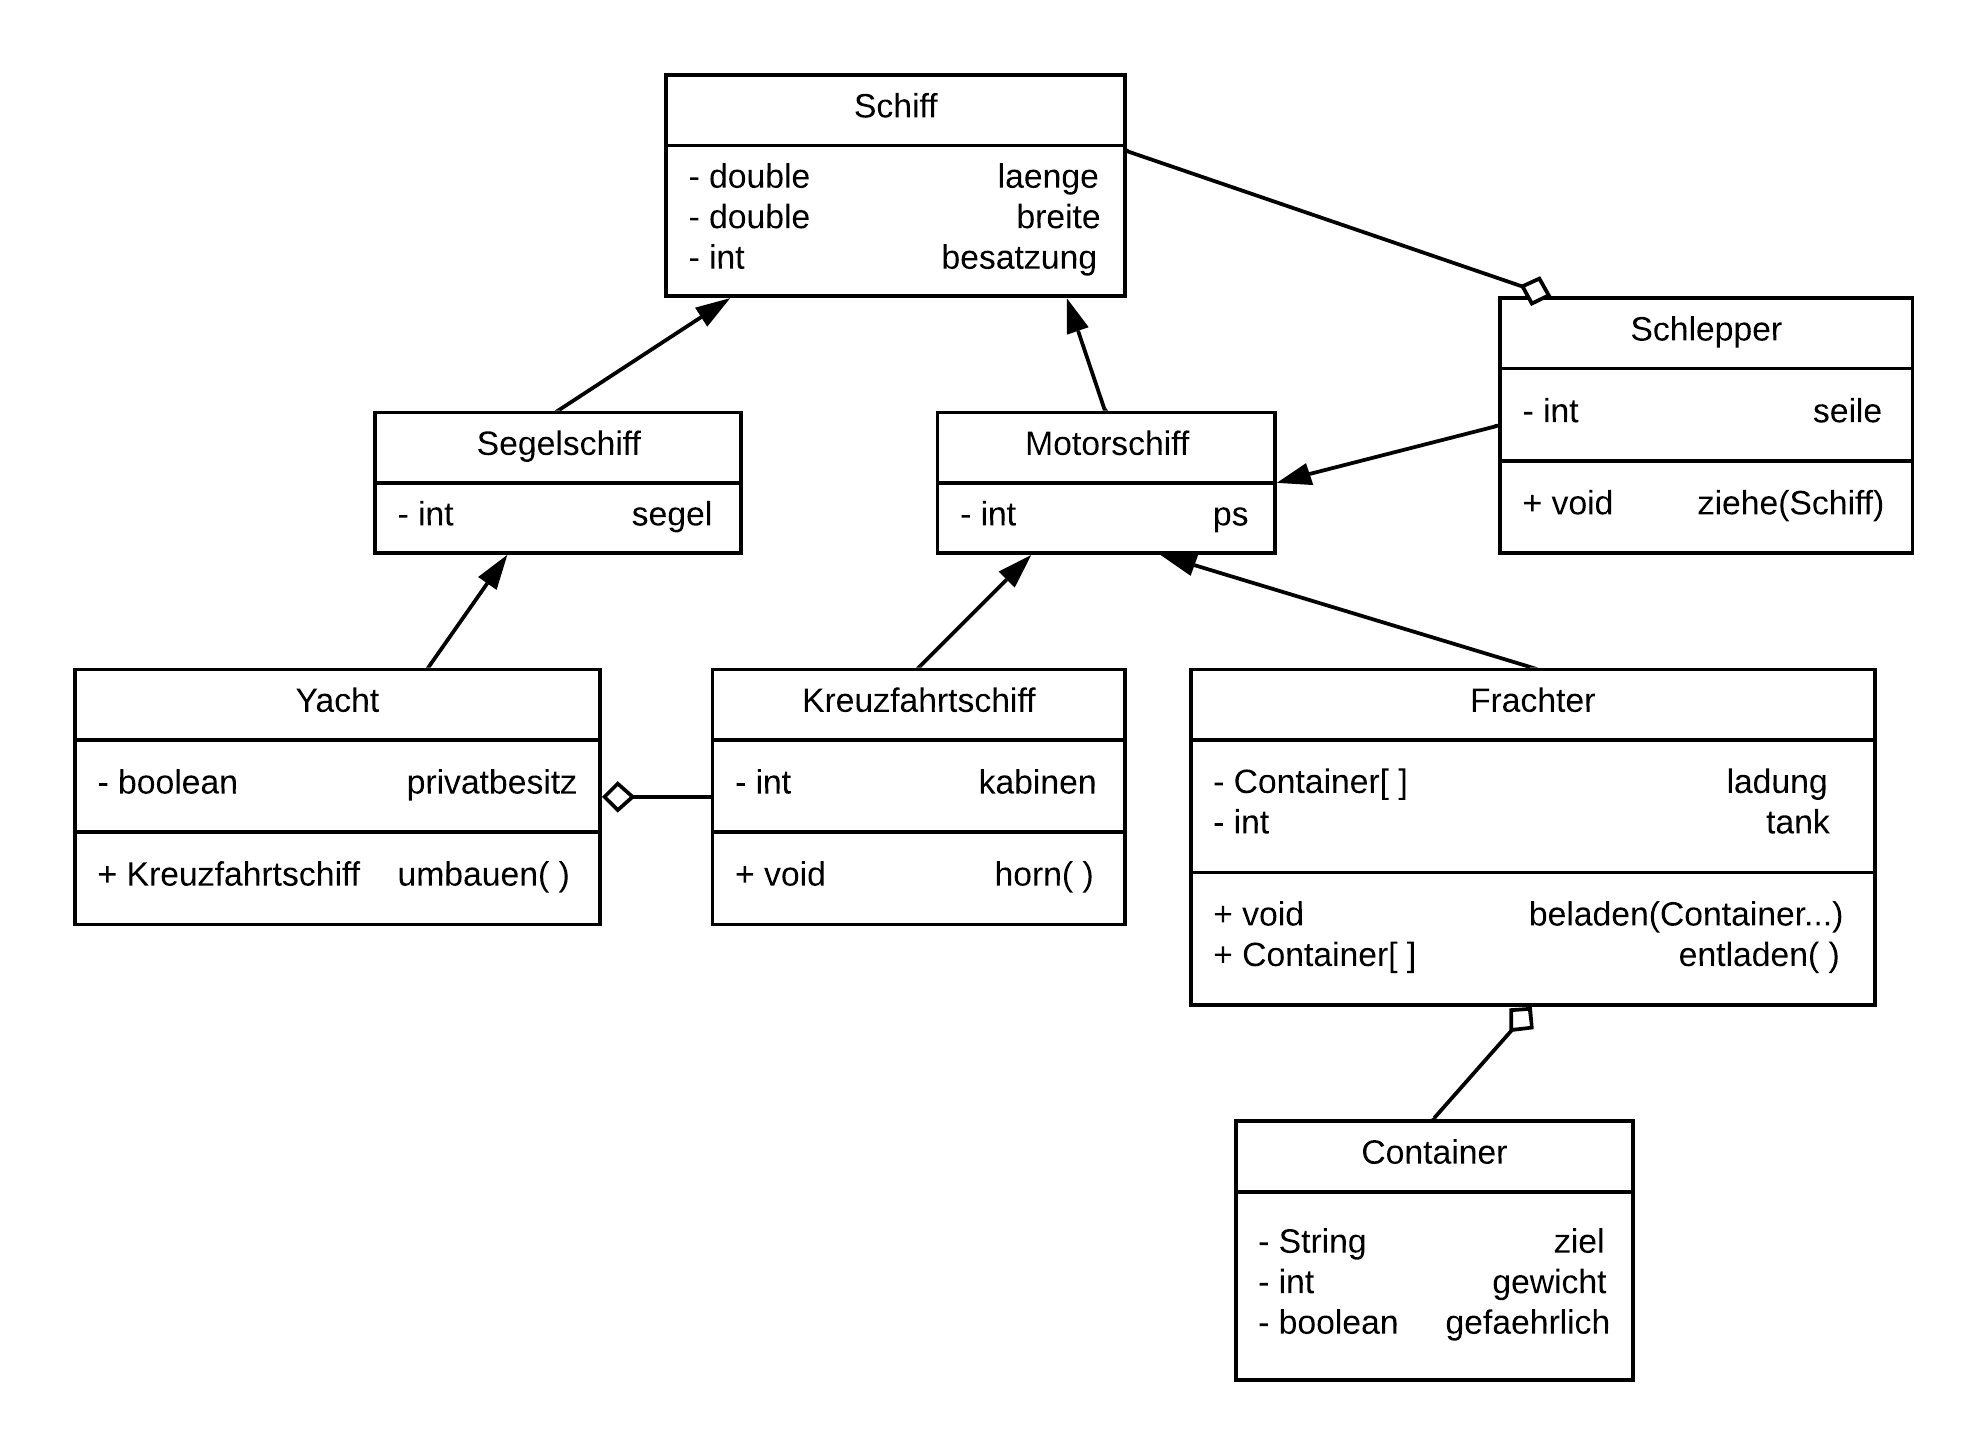
\includegraphics[width=1\textwidth]{Klassendiagramm.png}

\section{6)}
\begin{center}
    Code von Maximilian Petri
\end{center}
\pagebreak

\section{4)}
\subsection{}
\subsubsection{}
\begin{center}
    A(100) ruft A(int) auf, da es der speziellste passende Konstruktor in der Klasse A ist.\\
    Dieser ruft anschließend impliziet super(), also den Konstruktor von Object auf.\\
    Anschließend wird A(String) mit ''written in A(int)'' vom A(int) expliziet aufgerufen.\\
    Die println Anweisung gibt ''v1.x: written in A(int)'' aus, da dieser Wert im vorherigen Konstruktoraufruf für dieses Objekt so gesetzt wurde.
\end{center}

\subsubsection{}
\begin{center}
    B(100) ruft B(int) auf, da es der spez. passende Konstruktor in der Klasse B ist.\\
    Da B von A erbt, wird als nächstes impliziet super(), was dem Kontruktor A() gleicht, ausgeführt.\\
    Dieser ruft anschließend der Konstruktor von Object impliziet auf.\\
    Nun wird noch expliziet der Konstruktor A(String) mit ''written in A()'' aufgerufen.\\
    Es wird nun noch B(String) mit ''written in B(int)'' ausgeführt.\\
    Dieser ruft nun den super(String), also A(String) mit ''written in B(String)'' auf.\\
    Die erste println Anweisung gibt ''v2.x: written in B(String)'' aus, da dies zuletzt durch den super Aufruf im B(String) geändert wurde. Da v2 vom Typ A ist und in Java public var verdeckt werden, wird die verdeckte var aus A verwendet. Java läßt es außerdem zu final var während des Konstruktor aufrufs ''mehrfach'' zu ändern.\\
    Die zweite println Anweisung gibt ''((B) v2).x: written in B(int)'' aus. Das ist der Wert, welcher im explizieten Aufruf des B(String) Konstruktors durch B(int) in B.x gesetzt wurde. Da dieses x das aus x verdeckt, wird hier das aus der U-Klasse verwendet.
\end{center}

\subsubsection{}
\begin{center}
    B(v2) ruft B(A), welcher den super-Konstruktor A() impliziet aufruft, welcher den super-Konstruktor von Object impliziet aufruft und anschließend expliziet den Kontruktor A(String) mit "written in A()" aufruft, welcher impliziet den Super-Konstrukor von Onject aufruft und A.x auf den übergebenen String setzt.\\
    Anschließend wird expliziet in B(A) B(String) aufgerufen, welcher explziet den super-Konstruktor A(String) mit "written in B(String) aufruft, sodass in A.x dieser String hineingeschrieben wird. Nun wird noch in B.x ''written in B(A)'' geschrieben.\\
    Die erste println-Anweisung gibt ''((A) v3).x: written in B(String)'' aus, da dieses x verdeckt ist und da dieses Objekt nun vom Typ A ist.\\
    Die zweite println-Anweisung gibt ''v3.x: written in B(A)'' zurück, da dies der Wert ist, welcher in diese Variable geschrieben wurde und man über das B Objekt auf diese Variable zugreift, welche A.x verdeckt.
\end{center}
\pagebreak

\subsubsection{}
\begin{center}
    B() ruft B() auf, welcher impliziet den Super-Konstruktor A() aufuruft, welcher anschließend implziet den Super-Konstruktor von Oject aufruft.\\
    Es wird nun expliziet der A(String) aufgerufen, welcher ''written in A()'' in A.x reinschreibt.\\
    Anschließend wird B(String) expliziet mit ''written in B()'' aufgerfuen.\\
    Dieser ruft expliziet den Super-Konstruktor (A String) mit ''written in B(String)'', welcher impliziet den Super-Konstruktor von Object ausführt und A.x auf den übergebenen String setzt. Nun wird noch in B.x ''written in B()'' geschrieben.\\
    Die erste println-Anweisung gibt ''((A) v4).x: written in B(String)'' aus, da dieses x verdecjt ist un da dieses Objekt vom Typ A ist.\\
    Die zweite println-Anweisung gibt ''v4.x: written in B()'' aus, da dies der Wert ist, welcheer in diese Variable geschrieben wurd und man über das B Objekt auf diese Variable zugreift, welche A.x verdeckt.
\end{center}

\subsection{}
\textbf{(1)} A.f(A) \quad \quad \textbf{(2)} A.f(A) \quad \quad \textbf{(3)} A.f(A) \quad \quad \textbf{(4)} B.f(A) \quad \quad \textbf{(5)} B.f(A)\\

\textbf{(6)} B.f(A) \quad \quad \textbf{(7)} B.f(A) \quad \quad \textbf{(8)} B.f(A) \quad \quad \textbf{(9)} B.f(B)


\end{document}